\subsection{Risultati sperimentali}
Proponiamo alcuni risultati sperimentali ottenuti dal package Python contenente gli algoritmi per il calcolo della bisimulazione massima che abbiamo presentato nelle sezioni precedenti. Innanzitutto illustreremo brevemente l'ambiente e gli strumenti con cui sono state prese le misurazioni. Dopodichè presenteremo i risultati in forma di grafici, e tenteremo di evidenziare le differenze tra i vari algoritmi.

\subsubsection{Hardware e strumenti per le misura}
I risultati sono stati misurati su un computer con sistema operativo \emph{CentOS Linux}, architettura x86\_64, processore \emph{Intel(R) Core(TM) i7-4790 CPU} (4 cores, 3.60GHz), e memoria RAM da 16 GB. Per ottenere le misurazioni è stato utilizzato il package Python \emph{timeit}, che presenta alcune caratteristiche che lo rendono un valido strumento per la misurazione del tempo di esecuzione \cite{pythondocs}:
\begin{itemize}
    \item Utilizza la più precisa funzione disponibile sulla piattaforma per la misurazione del tempo trascorso;
    \item Disabilita il \emph{garbage collector}, che potrebbe intervenire in un momento casuale della misurazione introducendo rumore nei risultati;
    \item Esegue lo script preso in esame molte volte (il numero è deciso dall'utilizzatore) in modo da ridurre il rumore dovuto a temporanei sovraccarichi della CPU o della RAM.
\end{itemize}

I dataset su cui abbiamo effettuato le misurazioni sono stati generati utilizzando alcune funzioni del package Python \emph{NetworkX} \cite{networkx}.

\subsubsection{Performance}
Per avere dati significativi considereremo dataset composti da grafi con caratteristiche particolari.
\begin{figure}
    \centering
    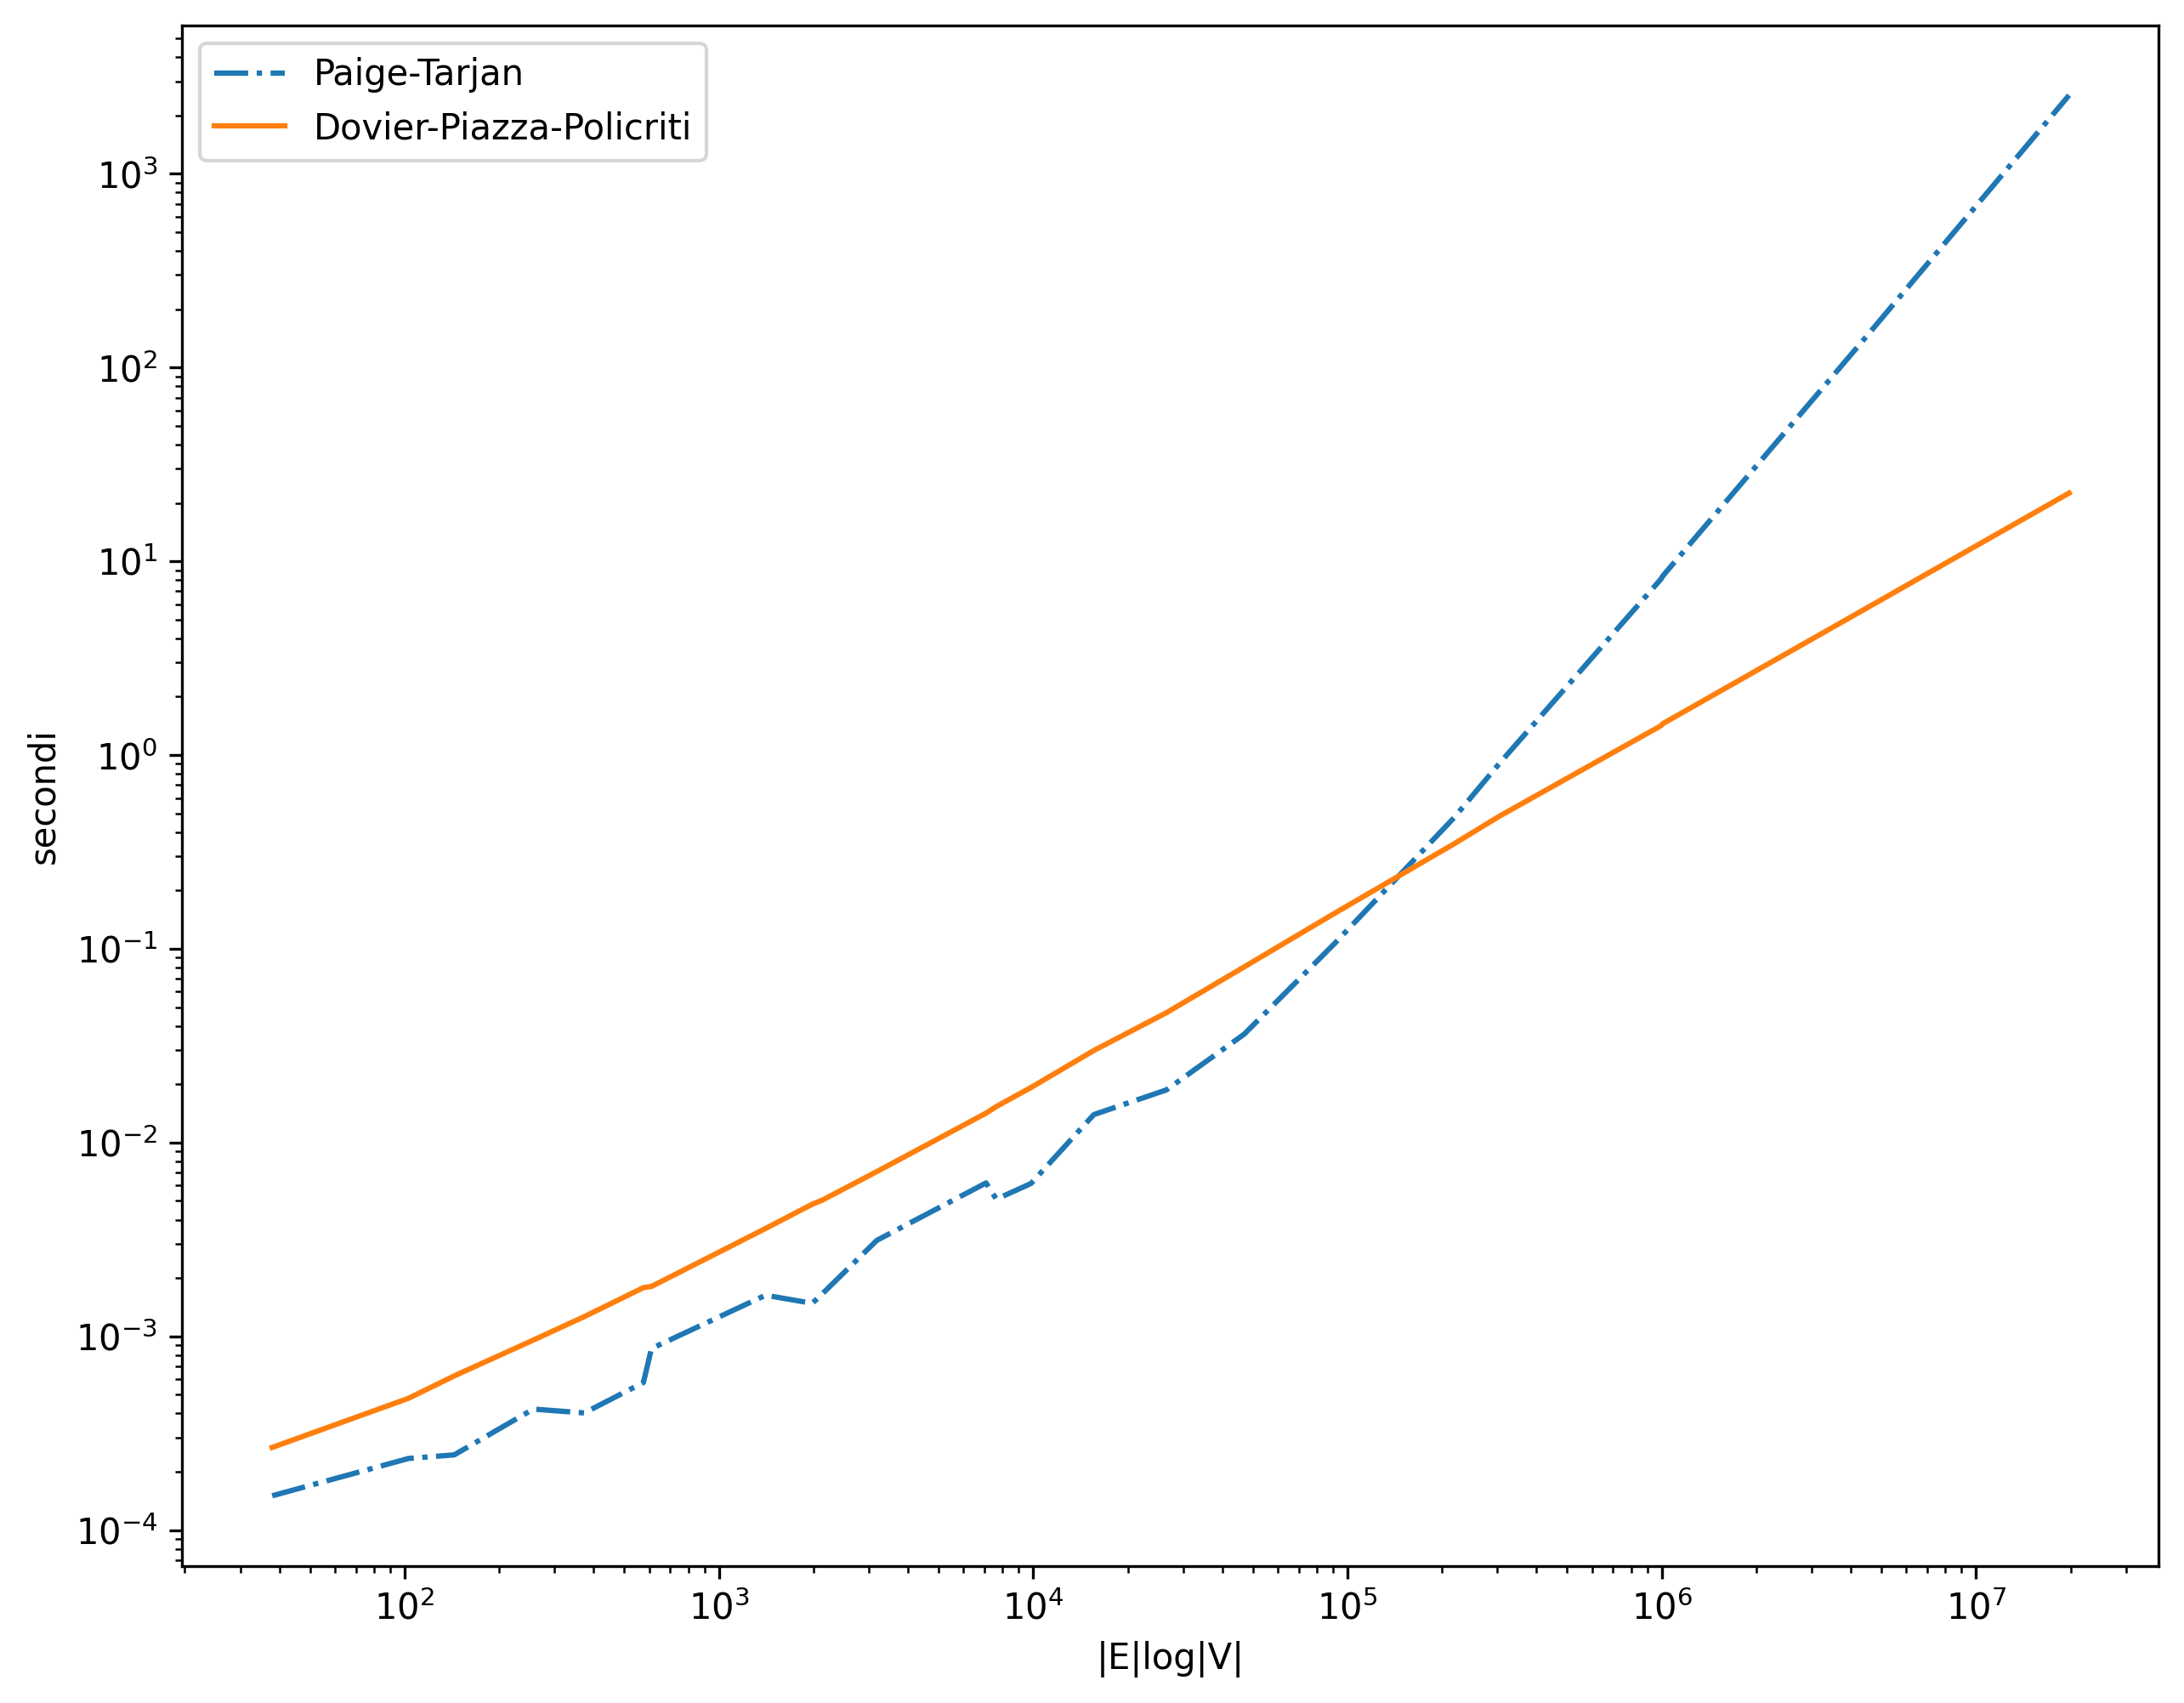
\includegraphics[width=0.7\textwidth]{./sezione3/experimental_results/plots/tree.png}
    \caption{Tempo di esecuzione degli algoritmi di \emph{Paige-Tarjan} (blu tratteggiato) e \emph{Dovier-Piazza-Policriti} (arancione continuo) su un dataset di ``alberi'' con \emph{depth} e \emph{branching-factor} variabili.}
    \label{fig:tree_exp_result}
\end{figure}

\subsubsection{Dimensione della bisimulazione massima}
Terminiamo la sezione relativa ai risultati sperimentali con un'ultima analisi che potrebbe essere di qualche interesse nella prospettiva di ciò che abbiamo presentato nella Sezione \ref{sec:applitations}. Consideriamo l'andamento del numero di classi di equivalenza nella bisimulazione massima per grafi di Erdős-Rényi (o \emph{grafi binomiali}), ovvero grafi contenenti un numero arbitrario \verb|n| di nodi, per cui presa una coppia qualsiasi $u,v \in V$ si ha $\langle u,v\rangle \in E$ con probabilità \verb|p| $< 1$.
Considereremo valori piccoli di \verb|p|, in quanto avvicinandoci ad 1 otteniamo grafi sempre più ``completi'' di interesse molto basso nella pratica.

\begin{figure}
    \makebox[\textwidth][c]{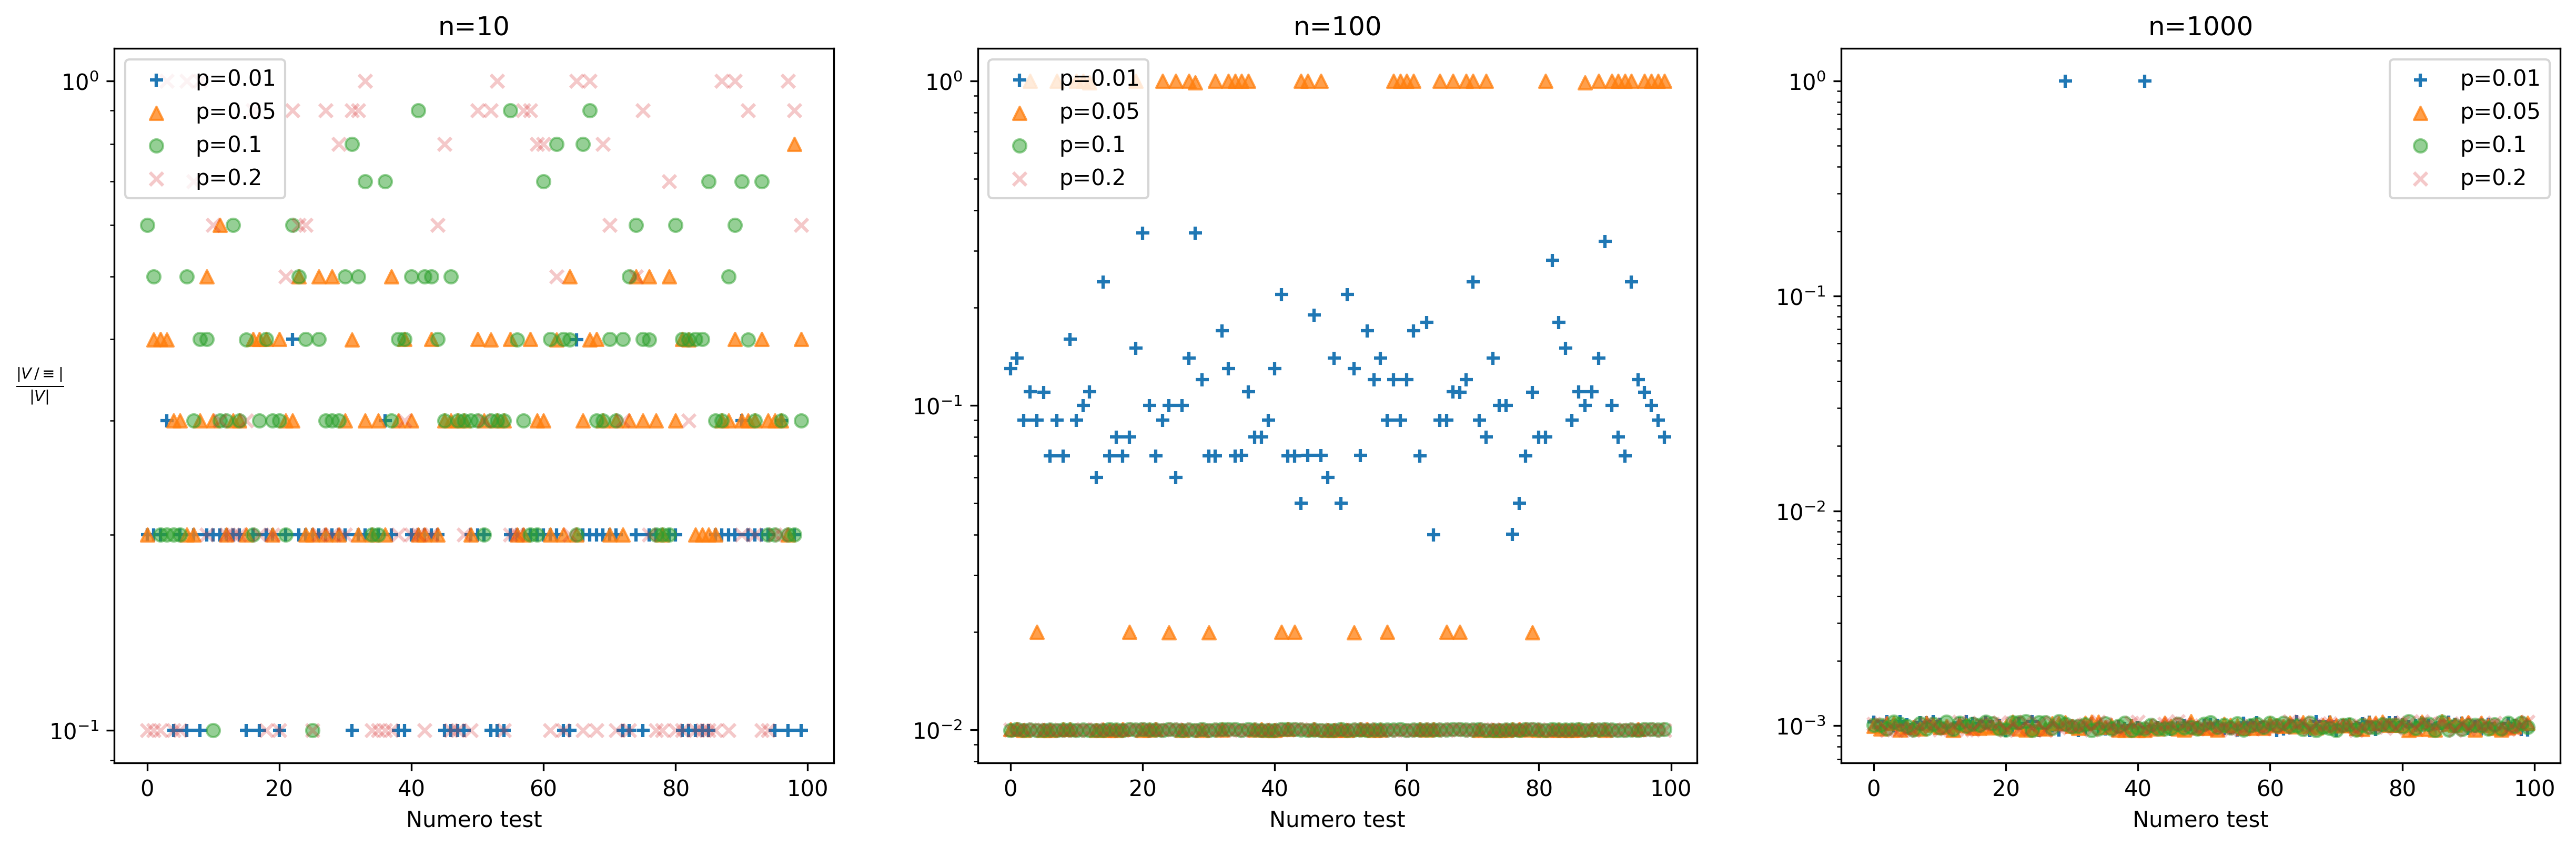
\includegraphics[width=1.2\textwidth]{./sezione3/experimental_results/plots/bisize.png}}
    \caption{Numero di classi di equivalenza della bisimulazione massima per grafi generati in modo casuale, normalizzato con il numero di nodi nel grafo.}
    \label{fig:bisi_size}
\end{figure}

Nella Figura \ref{fig:bisi_size} abbiamo tre diversi valori di \verb|n|, ed in ogni sotto-immagine abbiamo considerato i valori 0.01, 0.05, 0.1, 0.2 per \verb|p|. Per ogni combinazione di \verb|n|,\verb|p| abbiamo generato 100 grafi binomiali con la funzione \verb|fast_gnp_random_graph| del pacchetto \emph{NetworkX}, e ne abbiamo valutata la bisimulazione massima con l'algoritmo di \emph{Dovier-Piazza-Policriti}. Nei grafici abbiamo visualizzato la quantità $\frac{|V / \equiv|}{|V|}$, ovvero il rapporto tra il numero di classi di equivalenza nella bisimulazione massima ed il numero di nodi del grafo: questa quantità potrebbe essere considerata come il fattore di riduzione che otteniamo quanto sostuitiamo al grafo originale la sua contrazione secondo la bisimulazione massima.

Possiamo vedere in modo abbastanza evidente che per \verb|n=10| la quantità che stiamo valutando varia molto tra 1 (10 classi di equivalenza, nessuna riduzione) e 0.1 (tutti i nodi sono bisimili, riduzione massima). Per valori più grandi questa variabilità si riduce, e per \verb|n=1000| il fattore si schiaccia decisamente verso 0.001 (un'unica partizione).

Se la riduzione può essere un risultato positivo, bisogna anche considerare che con la riduzione abbiamo perso gran parte dell'informazione veicolata dal grafo originale. Infatti, se da 1000 nodi passiamo ad un solo nodo non vi può essere che un unico arco. A seconda delle applicazioni questa contrazione potrebbe risultare interessante o scoraggiante; si potrebbe tentare di correggere il risultato assegnando delle etichette ai nodi per imporre un partizionamento preventivo, che dovrà essere rispettato anche dalla bisimulazione massima.
